\documentclass[a4paper, 11pt]{report}
\usepackage[italian]{babel}
\usepackage[T1]{fontenc}
\usepackage[utf8]{inputenc}
\usepackage{amsmath}
\usepackage{amsfonts}
\usepackage{amsthm}
\usepackage{frontespizio}
\usepackage{hyperref}
\hypersetup{hidelinks,
	colorlinks = true,
	urlcolor = black, 
	linkcolor = black}
\usepackage[margin=3cm]{geometry}
\usepackage{booktabs}
\usepackage{fancyhdr}
\usepackage{listings}
\usepackage{stmaryrd}
\usepackage[strict]{changepage}
\usepackage{galois}
\usepackage{libertine}
\usepackage{textcomp}
\usepackage{float}
\usepackage{multicol}
\usepackage{makecell}
\usepackage{stmaryrd}
\usepackage{amssymb}
\renewcommand\theadalign{bc}
\renewcommand\theadfont{\bfseries}
\renewcommand\theadgape{\Gape[4pt]}
\renewcommand\cellgape{\Gape[4pt]}

\lstset{basicstyle=\ttfamily\small}

\newcommand{\parts}[1]{\mathcal{P}(#1)}
\newcommand{\galoistuple}{\langle C, \alpha, \gamma , A \rangle}

\newtheorem{definit}{Definizione}[subsection]
\newtheorem{thm}{Teorema}[subsection]

\begin{document}
	
\begin{frontespizio}
	\Preambolo{\usepackage{datetime}}
	\Istituzione{Università degli Studi di Verona}
	\Divisione{Dipartimento di informatica}
	\Titolo{Analisi dei Sistemi Informatici}
	\Scuola{}
	\Sottotitolo{Riassunto dei principali argomenti}
	\Candidato{Marco Colognese}
	\NCandidato{Autore}
	\Annoaccademico{2017/2018}
\end{frontespizio}
	
	
	
\tableofcontents
	
	\chapter*{Interpretazione Astratta}
	\addcontentsline{toc}{chapter}{Interpretazione Astratta}
	
	\section*{Accelerazione della convergenza}
	\addcontentsline{toc}{section}{Accelerazione della convergenza}
	\subsection*{Widening}
	\addcontentsline{toc}{subsection}{Widening}
	Un widening \[ \nabla : P \times P \to P  \] su un poset $ \langle P, \leq_P \rangle $ è una funzione che soddisfa:
	\begin{itemize}
		\item $\forall x,y \in P : x \sqsubseteq (x \nabla y ) \wedge y \sqsubseteq (x \nabla y)$
		\item per ogni catena ascendente $x_0 \sqsubseteq x_1 \sqsubseteq ... \sqsubseteq x_n$ la catena definita come $y_0 = x_0, ..., y_{n+1} = y_n \nabla x_{n+1}$ non è strettamente crescente.
	\end{itemize}
	
	Dato che in interpretazione astratta è necessario garantire/accelerare la convergenza, viene usato il widening (che si sostituisce al least upper bound), dal momento che anche il calcolo astratto può divergere.
	Il risultato di un widening è un post-puntofisso  di $F^\nabla$, ovvero una sovra-approssimazione del punto fisso più piccolo di f $lfp^\sqsubseteq F$. 
	
	Ad esempio, il widening su intervalli funziona come segue:
	\begin{align*}
	\lbrack a, b \rbrack\ \nabla\ \lbrack c, d \rbrack = \lbrack e, f \rbrack \qquad \text{ tale che}
	\end{align*}
	
	\begin{align*}
	e = 
	\begin{cases}
	-\infty &\text{ se } c < a \\
	a &\text{ altrimenti}
	\end{cases}
	\text{ e } f = 
	\begin{cases}
	+\infty &\text{ se } b < d\\
	b &\text{ altrimenti }
	\end{cases}
	\end{align*}
	
	\subsection*{Narrowing}
	\addcontentsline{toc}{subsection}{Narrowing}
	Dato che il widening raggiunge un post-fixpoint, piuò capitare che si abbiano eccessive perdite di informazione, in questo caso viene usato il narrowing.
	
	\begin{definit}
		Il narrowing è una funzione $ \triangle : P \times P \to P$ tale che:
		\begin{itemize}
			\item $\forall x, y \in \mathcal{P}: y \leq x \implies y \leq x\ \triangle\ y \leq x$
			\item Per ogni catena discendente $x_0 \geq x_1 \geq ...$, la catena discendente $y_0=x_0, ..., y_{i+1} = y_i\ \triangle\ x_{i+1}$ non è strettamente decrescente.
		\end{itemize}
	\end{definit}
	
	Per gli intervalli il narrowing funziona come segue:
	\begin{align*}
	\lbrack a, b \rbrack\ \triangle\ \lbrack c, d \rbrack = \lbrack e, f \rbrack \qquad \text{ tale che}
	\end{align*}
	\begin{align*}
	e = 
	\begin{cases}
	c &\text{ se } a = -\infty \\
	a &\text{ altrimenti}
	\end{cases}
	\text{ e } f = 
	\begin{cases}
	d &\text{ se } b = +\infty\\
	b &\text{ altrimenti }
	\end{cases}
	\end{align*}
	
	\section*{Correttezza}
	\addcontentsline{toc}{section}{Correttezza}
	Consideriamo $C \galois{\alpha}{\gamma} A$, una funzione concreta $f: C\rightarrow C$ e una funzione astratta $f^{\sharp}: A\rightarrow A$. Possiamo dire che $f^{\sharp}$ è un'approssimazione corretta di f in A se:
	\begin{equation*}
	\forall c\in C: \alpha(f(c))\leq_A f^{\sharp}(\alpha(c))
	\end{equation*}
	
	\noindent
	oppure, equivalentemente:
	\begin{equation*}
	\forall a\in A: f(\gamma(a))\leq_C \gamma(f^{\sharp}(a))
	\end{equation*}
	
	Nel processo di astrazione è ammessa una perdita di informazioni, ciò non è possibile nel processo di concretizzazione, dunque possiamo dire che se $c\in C$. Possiamo  dire che $\alpha(c)$ è l'elemento astratto più preciso che rappresenta \textit{c}.
	
	\begin{multicols}{2}	
		\begin{figure}[H]
			\centering
			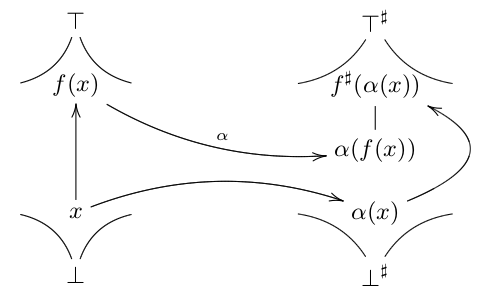
\includegraphics[scale=0.35]{Correttezza}
			\caption{Condizione di correttezza: $\alpha(f(c))\leq_A f^{\sharp}(\alpha(c))$}
			\label{Correct}
		\end{figure}
		\columnbreak
		\begin{figure}[H]
			\centering
			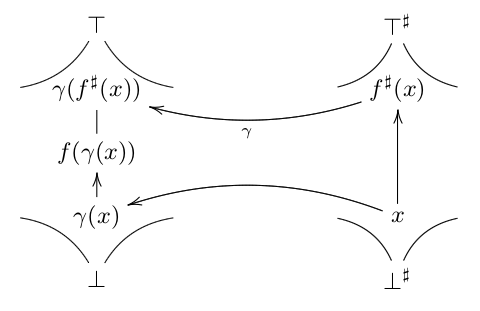
\includegraphics[scale=0.35]{CorrettezzaAstr}
			\caption{Condizione di correttezza: $f(\gamma(a))\leq_C \gamma(f^{\sharp}(a))$}
			\label{CorrectAbstr}
		\end{figure}
	\end{multicols}
	
	\section*{Completezza}
	\addcontentsline{toc}{section}{Completezza}
	Consideriamo $C \galoiS{\alpha}{\gamma} A$, una funzione concreta $f: C\rightarrow C$ e una funzione astratta $f^{\sharp}: A\rightarrow A$. Possiamo dire che:
	\begin{itemize}
		\item $f^{\sharp}$ è backward-complete per f se: $\forall c\in C: \alpha(f(c))=f^{\sharp}(\alpha(c))$;
		\item $f^{\sharp}$ è forward-complete per f se: $\forall a\in A: f(\gamma(a))=\gamma(f^{\sharp}(a))$.
	\end{itemize}
	
	I due tipi di completezza rappresentano una situazione in cui non si verifica nessuna perdita di precisione durante l'astrazione. In particolare:
	\begin{itemize}
		\item La \textbf{B}-completezza considera l'astrazione sull'output delle operazioni e non si accumula nessuna perdita di precisione astraendo in \textit{p} gli argomenti di \textit{f};
		\item La \textbf{F}-completezza considera l'astrazione sull'input delle operazioni e non si accumula nessuna perdita di precisione approssimando il risultato della funzione \textit{f} calcolata in \textit{p}.
	\end{itemize}
	
	\begin{multicols}{2}	
		\begin{figure}[H]
			\centering
			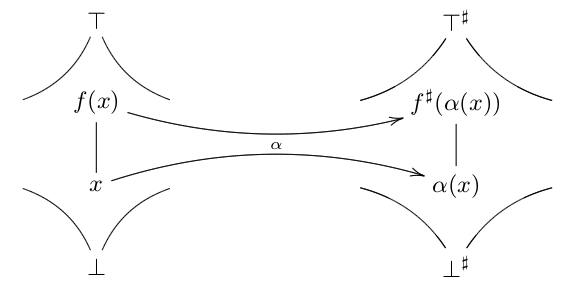
\includegraphics[scale=0.33]{Backward}
			\caption{Condizione di \textit{\textbf{B}-completezza}}
			\label{Backward}
		\end{figure}
		\columnbreak
		\begin{figure}[H]
			\centering
			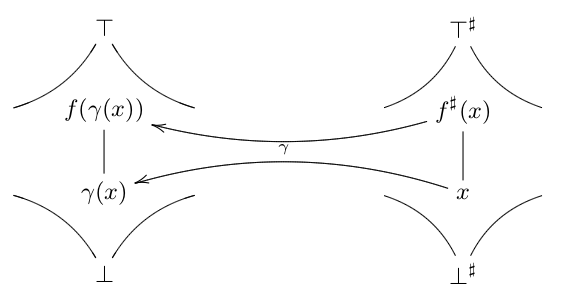
\includegraphics[scale=0.33]{Forward}
			\caption{Condizione di \textit{\textbf{F}-completezza}}
			\label{Forward}
		\end{figure}
	\end{multicols}

	\section*{Linguaggio e semantica}
	\addcontentsline{toc}{section}{Linguaggio e semantica}
	Introduciamo in questa sezione il linguaggio che verrà usato nel resto della dispensa e la sua semantica.
	
	\begin{center}
		\begin{tabular}{cc}
			\hline
			\textbf{Statement} & \textbf{Codice} \\
			\hline
			\hline
			Variabili & \lstinline|x| \\
			Espressioni aritmetiche & \lstinline|e| \\
			Assegnamenti & $x \leftarrow e$ \\
			Lettura da memoria & $x \leftarrow M[e]$ \\
			Scrittura in memoria & $M[e]_1 \leftarrow e_2$ \\
			Condizionali & \lstinline|if (e) S|$_1$ \lstinline|else S|$_2$ \\
			Salto non condizionale & \lstinline|goto L|\\
			\hline
		\end{tabular}
	\end{center}
	
	La memoria $M$ è vista come un array arbitrariamente grande dove i valori possono essere inseriti e letti.
	
	\begin{itemize}
		\item $x$ e $M[e]$ sono contenitori di valori;
		\item il contenuto di $M[e]$ non è visibile fino alla valutazione di $e$;
		\item $x$ è solamente il nome tramite cui accedere al contenitore associato.
	\end{itemize}


	
	\section*{Collecting Semantics}
	\addcontentsline{toc}{section}{Collecting Semantics}
	\MakeUppercase{è} l'insieme dei comportamenti osservabili nella semantica operazionale. La \textit{Collecting Semantics} è il punto di partenza per ogni tipo di analisi (non ne esiste una universale).
	
	La \textbf{\textit{trace semantics}} di un programma accumula informazioni temporali riguardo l'esecuzione: una traccia tiene conto dell'ordine in cui i \textit{program states} sono raggiunti durante l'esecuzione.
	\noindent
	Le tracce analizzate possono essere dei seguenti tipi:
	\begin{itemize}
		\item L'insieme di tutti i discendenti dello stato iniziale.
		\item L'insieme di tutti i discendenti dello stato iniziale che può raggiungere uno stato finale.
		\item Lo stato di tutte le tracce finite dallo stato iniziale.
		\item L'insieme di tutte le tracce infinite e finite dallo stato iniziale ecc.
	\end{itemize}
	
	Però non sempre siamo interessati alle informazioni temporali ma solamente agli invarianti presenti ad ogni \textit{program point}. Questi invarianti possono essere astratti dalle informazioni temporali attraverso la \textbf{\textit{collecting semantics}}.
	
	Più formalmente, un invariante del programma $P$ al punto di programma $l$ è una qualsiasi proprietà $I\in P$ (store) che è presente ogni talvolta che $l$ viene raggiunto.
	
	La \textit{collecting semantics} di $P$ è semplicemente l'associazione tra i vari \textit{program point} e le corrispondenti invarianti ben precise.
	
	Lo stato di input non è noto al momento della compilazione, quindi vengono collezionati tutti gli stati raggiungibili da tutti i possibili ingressi del programma.
	\newline
	
	Si tratta di una collezione di stati che possono apparire su alcune tracce nei diversi program point. Trattandosi di un'astrazione, non è più possibile risalire alle tracce di esecuzione del programma conoscendo solamente i vari \textit{program states}.
	\begin{figure}[H]
		\centering
		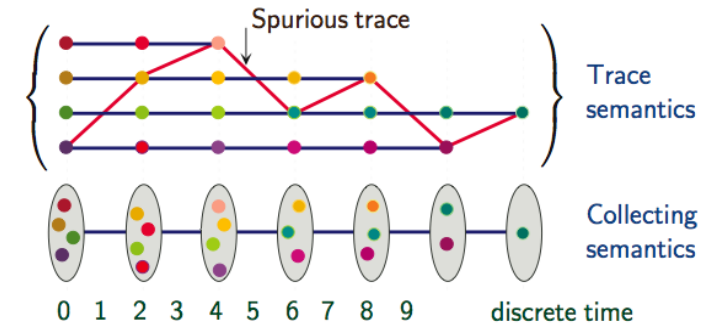
\includegraphics[scale=0.32]{TraceCollect}
		\caption{Esiste la traccia rossa? \textit{Trace semantics}: NO; \textit{collecting semantics}: NON LO SO.}
	\end{figure}
	
	
	
	\section*{Control-Flow-Graph (CFG)}
	\addcontentsline{toc}{section}{Control-Flow-Graph (CFG)}
	E costituito da:
	\begin{itemize}
		\item \textbf{nodi}: corrispondono ai \textit{program points};
		\item \textbf{archi}: passi di computazione etichettati con la corrispondente azione; sono della forma $K=(u, lab, v)$, dove $u$ è il nodo sorgente, $v$ è il nodo di destinazione e $lab$ è l'etichetta.
	\end{itemize}	
		\begin{center}
			\begin{tabular}{cc}
				\hline
				Test & $NonZero(e)$ or $Zero(e)$ \\
				Assegnamenti & $x \leftarrow e$ \\
				Lettura da memoria & $x \leftarrow M[e]$ \\
				Scrittura in memoria & $M[e]_1 \leftarrow e_2$ \\
				Statement vuoto & $;$ \\
				\hline
			\end{tabular}
		\end{center}

Ogni passo di computazione della semantica operazionale trasforma gli stati del programma:
\begin{equation*}
(\rho, \mu) \textnormal{ dove } \rho: Var \to int \textnormal{ e } \mu : \mathbb{N} \to int
\end{equation*}
\begin{itemize}
	\item La funzione $\rho$ mappa le variabili del programma al loro valore attuale;
	\item la funzione $\mu$ mappa ogni cella dell'array al suo contenuto nelle celle di memoria.
\end{itemize}

Una \textit{computazione} è un percorso che và da un nodo di partenza $u$ e termina in un nodo $v$. Il percorso è un insieme di archi del $CFG$. La trasformazione dello stato è data dalla composizione degli effetti degli archi.

\begin{equation*}
	\llbracket \pi\rrbracket\hspace{0.01cm} = \llbracket k_n\rrbracket \circ ... \circ \llbracket k_1\rrbracket
\end{equation*}
 
 Il \textbf{Control Flow Graph} è generato dalla sintassi del programma ed è utile per capire la struttura del codice.
 
 Viene utilizzato per effettuare \textit{debugging}, \textit{testing} ed individuare \textit{dead code}.
 
 \newtheorem*{definit1}{Basic Block}
 \begin{definit1}
	Sequenza massima di statements consecutivi con un singolo \textit{entry point}, un singolo \textit{exit point} e nessun \textit{branch} interno.
 \end{definit1}

I \textit{basic block} si identificano facilmente poiché iniziano con un \textit{leader} che può essere dei seguenti tipi:
\begin{itemize}
	\item l'\textit{entry point} del programma (il primo statement);
	\item ogni statement che è target di branch (condizionali o non condizionali) che contengono dei \textit{GoTo}
	\item ogni statement che segue un branch (condizionale o non condizionale) o un \textit{return}.
\end{itemize}

Dopo aver diviso il codice in \textit{basic block} (individuati tramite i \textit{leader} di ciascun blocco), essi verranno collegati dagli archi, in corrispondenza di:
\begin{itemize}
	\item \textit{GoTo} non condizionali;
	\item branch condizionali / archi multipli;
	\item flusso di programma (il controllo passa ad un altro blocco se non ci sono branch alla fine).
\end{itemize}

Se non c'è un unico \textit{entry-node} $n_0$ ed un unico \textit{exit-node} $n_f$, si aggiungono \textit{dummy nodes} e gli archi necessari (nessun arco entrante in $n_0$ e nessun arco uscende da $n_f$).

\subsection*{Notazione dei CFG}
\addcontentsline{toc}{subsection}{Notazione dei CFG}
Dato un $CFG$ $=$ $<N, E>$:
\begin{itemize}
	\item Se c'è un arco $n_in_j\in E$:
	\begin{itemize}
		\item $n_i$ è \textit{predecessore} di $N_j$;
		\item $n_j$ è un \textit{successore} di $n_i$.
	\end{itemize}
	\item Per ogni nodo $n\in N$:
	\begin{itemize}
		\item textit{Pred(n)}: è l'insieme dei predecessori di $n$;
		\item textit{Succ(n)}: è l'insieme dei successori di $n$;
		\item un \textit{branch node} è un nodo che ha più di un successore;
		\item un \textit{join node} è un nodo che ha più di un predecessore; 
	\end{itemize}
\end{itemize}

\newtheorem*{definit2}{Depth First Traversal}
\begin{definit2}
	Il CFG è un grafo diretto e con radice (entry-node). Deve essere attraversato partendo dalla radice ed esplorando in profondità il più possibile ciascun ramo prima di fare backtracking.
	
	E' possibile costruire uno \textbf{spanning tree} per il grafo che contenga tutti i nodi, tale che:
	\begin{itemize}
		\item ci sia un percorso dalla radice ad ogni nodo che sia raggiungibile nel grafo originale;
		\item non devono esserci cicli.
	\end{itemize}
\end{definit2}

\noindent
I nodi vengono numerati nell'ordine in cui verranno visitati.
\newpage
\begin{multicols}{2}	
	\begin{figure}[H]
		\centering
		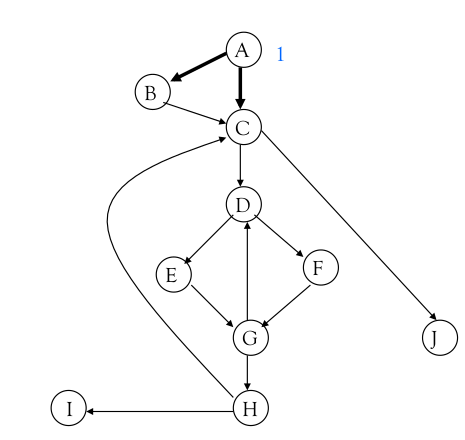
\includegraphics[scale=0.25]{SPT1}
	\end{figure}
\columnbreak
	\begin{figure}[H]
		\centering
		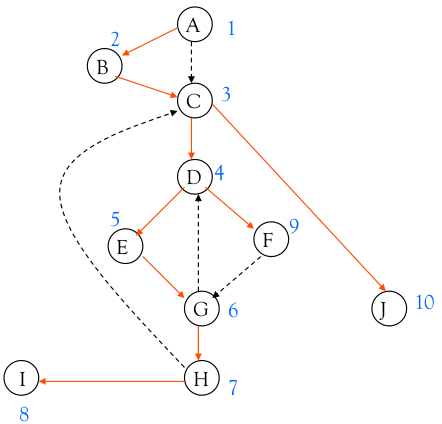
\includegraphics[scale=0.25]{SPT2}
	\end{figure}
\end{multicols}



\newtheorem*{definit3}{Classificazione degli archi}
\begin{definit3}
	Dato un arco $x \rightarrow y$ in un CFG, esso sarà:
	\begin{itemize}
		\item un \textbf{arco avanzante}: se $x$ è predecessore di $y$ nell'albero;
		\begin{itemize}
			\item \textbf{tree edge}: se è parte dello spanning tree;
			\item \textbf{forward edge}: se non è parte dello spanning tree e $x$ è predecessore di $y$ nell'albero.
		\end{itemize}
		\item un \textbf{arco all'indietro}: se $y$ è un predecessore di $x$ nell'albero;
		\item un \textbf{cross edge}: se non è parte dello spanning tree e nessun nodo è predecessore dell'altro.
	\end{itemize}
	\begin{figure}[H]
		\centering
		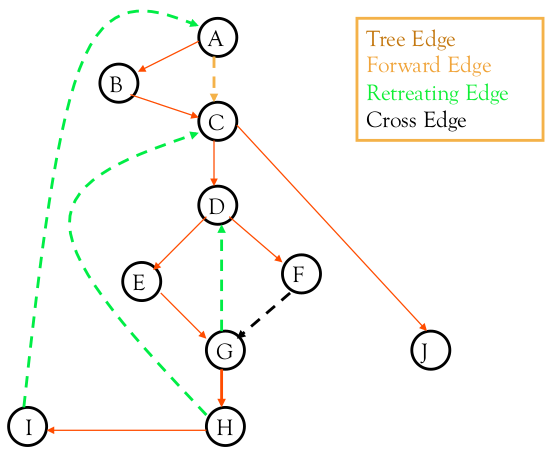
\includegraphics[scale=0.27]{Edges}
	\end{figure}
\end{definit3}

\newtheorem*{definit4}{Extended Basic Block}
\begin{definit4}
	Insieme massimo di nodi che non contiene nessun nodo di join (oltre all'entry node). Ha un solo ingresso e più uscite.
\end{definit4}

\newtheorem*{definit5}{Natural Loop}
\begin{definit5}
	Un Loop è un insieme di nodi strettamente connessi. Ha un unico ingresso (l'unico modo per visitarlo). Deve contenere un unico arco all'indietro per ripercorrere il loop.
	
	Un loop che non contiene altri loops è un \textit{inner loop}.
\end{definit5}
\noindent
Per trovare un loop all'interno di un grafo è sufficiente cercare gli archi all'indietro ($n\rightarrow d$).
\newline
Per costruire un loop si aggiunge $d$, si aggiunge $n$ (se $n\neq d$), si considera ogni nodo $m\neq d$ all'interno del loop (inserendo tutti i predecessori di $m$).
\newline

\begin{figure}[H]
	\centering
	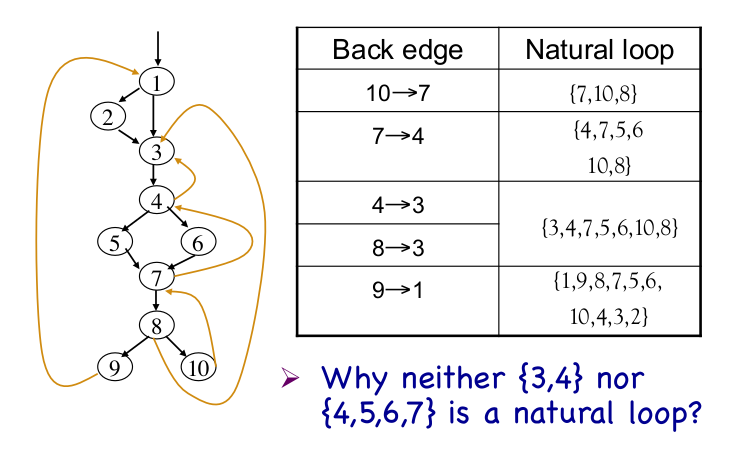
\includegraphics[scale=0.27]{NaturalLoop}
	\caption{Natural loops example}
\end{figure}

\newtheorem*{definit6}{Dominance}
\begin{definit6}
	Un nodo $d$ domina un nodo $n$ se ogni percorso dall'entry node del grafo fino a $n$ passa attraverso $d$ $(d$ \textit{dom} $n)$.
\end{definit6}
\begin{itemize}
	\item \textit{Dom(n)}: l'insieme dei dominatori del nodo $n$;
	\item ogni nodo domina se stesso: $n\in Dom(n)$;
	\item il nodo $d$ domina strettamente $n$ se $d\in Dom(n)$ e $d\neq n$;
	\item \textit{Dominance-based loop recognition}: la entry di un loop domina tutti i nodi interni al loop.
\end{itemize}

Ogni nodo $n$ ha un unico \textit{dominatore immediato} $m$ che è l'ultimo dominatore di $n$ su ogni percorso dall'entry node a $n$ $(m$ \textit{idom} $n)$, $m\neq n$.

\begin{figure}[H]
	\centering
	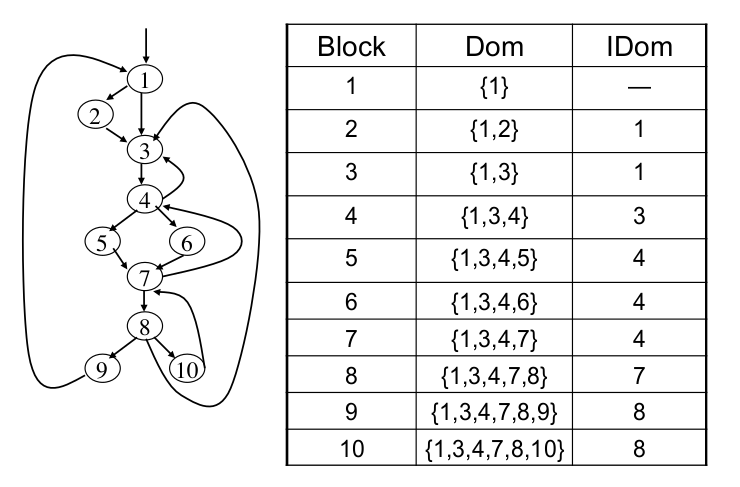
\includegraphics[scale=0.32]{DominatorExample}
	\caption{Dominator example}
\end{figure}



\chapter*{Analisi Statica}
\addcontentsline{toc}{chapter}{Analisi Statica}

\section*{Introduzione}
\addcontentsline{toc}{section}{Introduzione}
L'obiettivo dell'analisi statica è quello di dire, osservando le proprietà semantica di un programma, se una certa proprietà vale o meno. Esistono diverse tipologie di analisi statica: \begin{itemize}
	\item Control flow Analysis;
	\item Data flow Analysis (distributive e non-distributive);
\end{itemize}

\section*{Analisi sul CFG}
\addcontentsline{toc}{section}{Analisi sul CFG}
Viene generato un CFG per ogni procedura. Le analisi che vengono eseguite sono localizzate a 3 livelli: \begin{enumerate}
	\item \textbf{Locali al blocco}: sono eseguite all'interno di uno stesso \textit{basic block};
	\item \textbf{Intra-procedurali}: considerano il flusso di informazioni nel singolo CFG;
	\item \textbf{Inter-procedurali}: considerano il flusso di informazioni tra le procedure (con archi che rappresentano le chiamate di funzione).
\end{enumerate}

\noindent
L'analisi di \textit{data-flow} dice come l'informazione viene manipolata in un blocco. L'informazione è caratterizzata dalla soluzione dell'equazione di punto fisso definita per ogni blocco.

\noindent
In alcuni casi questa equazione è ottenuta in 3 passaggi: \begin{itemize}
	\item definendo l'informazione entrante in un blocco, che è l'unione dell'informazione di uscita del blocco precedente;
	\item definendo l'informazione in uscita dal blocco che è l'informazione in ingresso, modificata dalle operazioni eseguite nel blocco;
	\item queste definizioni vengono poi combinate nell'equazione del punto fisso.
\end{itemize}

Le analisi di \textit{data-flow} seguono il seguente schema:
\begin{figure}[H]
	\centering
	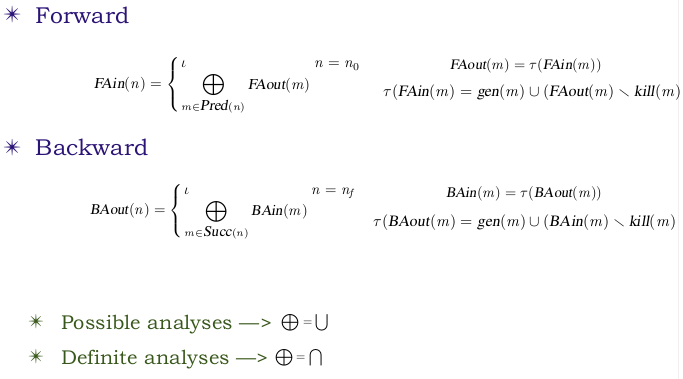
\includegraphics[scale=0.376]{FB}
\end{figure}

\newpage
\section*{Soluzioni MFP - MOP - IDEAL}
\addcontentsline{toc}{section}{Soluzioni MFP - MOP - IDEAL}
Per le equazioni di \textit{data-flow analysis} esistono 3 tipi di soluzioni:
\begin{itemize}
	\item \textit{\textbf{MFP} (maximum fixed point)}: è la soluzione che combina i valori dell'analisi quando il CFG ha dei nodi in cui convergono due o più percorsi; questa soluzione approssima la \textit{MOP}.
	\item \textit{\textbf{MOP} (merge over all paths)}: è la soluzione più precisa rispetto alla \textit{MFP} ($MOP \sqsupseteq MFP$) poiché combina i valori dell'analisi di tutti i possibili percorsi del CFG dopo averli attraversati tutti. In generale, questa soluzione non è computabile perché ci posso essere un numero esponenziale (o infinito) di percorsi possibili:
	\begin{itemize}
		\item loop con guardia sempre vera;
		\item un programma che contiene $N$ \textit{if} statement avrà $2^N$ percorsi di esecuzione;
	\end{itemize}
	\item \textbf{\textit{IDEAL}}: è la soluzione migliore ma non è computabile. A differenza della \textit{MOP}, prende in considerazione solamente i percorsi che verrano attraversati sicuramente da almeno qualche esecuzione. Calcola il valore alla fine di ogni possibile percorso di esecuzione e calcola poi il \textit{meet} di questi valori.
	\begin{itemize}
		\item ogni soluzione più grande di \textit{IDEAL} è scorretta;
		\item ogni soluzione più piccola di \textit{IDEAL} è conservativa (\textit{safe});
	\end{itemize}
\end{itemize}
Se la funzione di trasferimento di ogni arco è \textbf{\textit{distributiva}} ($f(x \cup y) = f(x) \cup f(y)$) (e ogni program point è raggiungibile dall'entry point), allora la soluzione delle equazioni di \textit{data-flow} è la stessa per \textit{MOP} e \textit{MFP} ($MOP = MFP$). Dunque per le funzioni di trasferimento distributive, è possibile calcolare la soluzione \textit{MOP} attraverso l'algoritmo iterativo del punto fisso.
\newline

I \textbf{problemi \textit{distributivi}} sono i cosiddetti problemi "\textit{semplici}", come ad esempio: \textit{\textbf{live variables}}, \textit{\textbf{available expressions}}, \textit{\textbf{reaching definitions}} e \textit{\textbf{very busy expressions}} (tutte proprietà che ci dicono \textit{COME} un programma viene eseguito).

I \textbf{problemi \textit{non-distributivi}} sono quelli che ci dicono \textit{COSA} calcola un programma (ad esempio che l'output è costante, valori positivi, intervalli etc.). Un esempio di problema non distributivo è la \textit{\textbf{constant propagation analysis}}.

\begin{multicols}{2}	
	\begin{figure}[H]
		\centering
		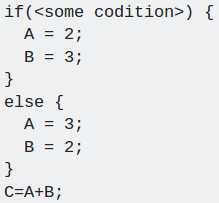
\includegraphics[scale=0.55]{MOPMFP}
	\end{figure}
	\columnbreak
	Se consideriamo la \textit{constant propagation}, in questo programma il valore ci $C$ sarà sempre $5$, indipendentemente dal valore della guardia dello statement \textit{if}.
	
	Con una soluzione \textit{MFP}, $C$ non verrà mai considerata una costante, al contrario, con una soluzione \textit{MOP} otterremo come informazione che la variabile $C$ è una costante.
\end{multicols}

\newpage
\section*{Data Flow Analysis}
\addcontentsline{toc}{section}{Data Flow Analysis}
Insieme di tecniche che raccolgono informazione su come i dati fluiscono durante l'esecuzione.

\subsection*{\underline{Problemi Distributivi}}
\addcontentsline{toc}{subsection}{Problemi Distributivi}

\subsubsection*{Available Expressions}
\addcontentsline{toc}{subsubsection}{Available Expressions}
L'espressione $e$ è \textit{available} se è valutata e assegnata ad una variabile prima di $v$ (uso della variabile). Tra la valutazione e $v$ non vengono ridefinite le variabili dell'espressione e \textit{x} (\textit{x:=e}).
\newline

\noindent
\textit{\underline{Proprietà}}: Forward \& Definite
\newline

\noindent
\underline{\textit{Punto fisso:}}
\begin{align*}
	AvailIn(n) &= 
	\begin{cases}
	\emptyset &\text{ se } n = n_0 \\
	\bigcap_{m\in pred(n)} AvailOut(m) &\text{ altrimenti}
	\end{cases}\\ \\
	AvailOut(n) &= Gen(n) \cup (AvailIn(n)\backslash Kill(n))\\
	AvailIn(n) &= \bigcap_{m\in pred(n)} Gen(m) \cup (AvailIn(m)\backslash Kill(m))
\end{align*}

\noindent
\underline{\textit{Semantica:}}

Dominio astratto = Ass = \{assegnamenti $x\leftarrow e ~|~ x\notin Var(e)$\}

$A\subseteq Ass$
\begin{align*}
	\llbracket ; \rrbracket^\sharp A &= A\\
	\llbracket NonZero(e) \rrbracket^\sharp A &= \llbracket Zero(e) \rrbracket^\sharp A = A\\
	\llbracket x\leftarrow e \rrbracket^\sharp A &= \begin{cases}
	(A\backslash Occ(x)) \cup \{x\leftarrow e \} &\text{ se } x\notin Var(e) \\
	A\backslash Occ(x) &\text{ altrimenti}
	\end{cases}\\
	\llbracket x\leftarrow M[e] \rrbracket^\sharp A &= A\backslash Occ(x)\\
	\llbracket M[e_1]\leftarrow e_2 \rrbracket^\sharp A &= A
\end{align*}

$Occ(x) = $ \{Assegnamenti che coinvolgono $x$ a destra o a sinistra\}

$Gen(n) = $ \{espressioni valutate nel blocco $n$ e nessun operando di $e$ è definito nuovamente tra l'ultima valutazione di $e$ in $n$ e la fine di $n$\}

$Kill(n) = $ \{espressioni uccise da una nuova definizione di $n$\}

\noindent


\newpage
\subsubsection*{Very Busy Expressions}
\addcontentsline{toc}{subsubsection}{Very Busy Expressions}
Un assegnamento è \textit{busy} su un cammino $\pi$ se $\pi = \pi_1 ~k~ \pi_2$ con:
\begin{itemize}
	\item $k$ è un assegnamento $x\leftarrow e$;
	\item $\pi_1$ non contiene usi di $x$;
	\item $\pi_2$ non contiene modifiche di $\{x\}\cup Var(e)$.
\end{itemize}

\noindent
Un assegnamento è \textit{very busy} se è \textit{busy} su ogni percorso da $v$ a \textit{exit}.

\noindent
Dice come e quali espressioni anticipare.

\noindent
Un assegnamento è ucciso in un blocco $n$ se una delle sue variabili è modificata o se $e$ viene usata.

\noindent
Un assegnamento è generato in un blocco $n$ se si trova nel blocco e l'espressione non contiene la variabile che si sta assegnando.
\newline

\noindent
\textit{\underline{Proprietà}}: Backward \& Definite
\newline

\noindent
\underline{\textit{Punto fisso:}}
\begin{align*}
VB_{exit}(p) &= 
\begin{cases}
\emptyset &\text{ se } p = v_{exit} \\
\bigcap_{q\in succ(p)} VB_{entry}(q) &\text{ altrimenti}
\end{cases}\\ \\
VB_{entry}(p) &= Gen(p) \cup (VB_{exit}(p)\backslash Kill(p))\\
VB_{exit}(p) &= \bigcap_{q\in succ(p)} Gen(q) \cup (VB_{exit}(q)\backslash Kill(q))
\end{align*}

\noindent
\underline{\textit{Semantica:}}

$B = 2^{Ass} = \mathcal{P}(Ass)$
\begin{align*}
\llbracket ; \rrbracket^\sharp B &= B\\
\llbracket NonZero(e) \rrbracket^\sharp B &= \llbracket Zero(e) \rrbracket^\sharp B = B \backslash Ass(e)\\
\llbracket x\leftarrow e \rrbracket^\sharp B &= \begin{cases}
B\backslash (Occ(x) \cup Ass(e)) \cup \{x\leftarrow e \} &\text{ se } x\notin Var(e) \\
B\backslash (Occ(x) \cup Ass(e)) &\text{ altrimenti}
\end{cases}\\
\llbracket x\leftarrow M[e] \rrbracket^\sharp B &= B\backslash (Occ(x) \cup Ass(e))\\
\llbracket M[e_1]\leftarrow e_2 \rrbracket^\sharp B &= B\backslash (Ass(e_1) \cup Ass(e_2))
\end{align*}

$Use(n) = $ \{occorrenza di una variabile sul lato destro di uno statement\}

\newpage
\subsubsection*{Liveness}
\addcontentsline{toc}{subsubsection}{Liveness}
$x$ è \textit{live} all'uscita del blocco $b$ se verrà usata successivamente. $x$ non è \textit{live} o (\textit{dead}) se viene ridefinita prima di un successivo uso.

\noindent
$x$ è \textit{live} in un cammino $\pi$ ($v\rightarrow exit$) se:
\begin{itemize}
	\item $\pi$ non contiene \textit{Def(x)} e,
	\item esiste almeno un uso di $x$ in $\pi$ che segue la \textit{Def(x)};
\end{itemize}
\noindent
$x$ è \textit{live} se si trova tra una definizione ed un uso.

\noindent
Dice se $a$ e $b$ possono essere memorizzate nella stessa locazione, cioè se $a$ e $b$ non sono mai \textit{live} insieme, allora posso sostituire $a$ con $b$.

\begin{itemize}
	\item $x\in Use(n) \Rightarrow$ x \textit{LiveIn} in $n$
	\item $x$ è \textit{LiveOut} in $n$ e $x\notin$ \textit{VarKill(n)} $\Rightarrow$ $x$ \textit{LiveIn} in $n$;
	\item $x$ è \textit{LiveIn} in almeno un \textit{Succ(n)} $\Rightarrow$ $x$ \textit{LiveOut(n)};
\end{itemize}

\noindent
\textit{\underline{Falsi positivi}}:
\begin{itemize}
	\item $x$ è accessibile attraverso altri nomi $\Rightarrow$ Liveness fallisce;
	\item analizzi anche cammini non possibili;
	\item inizializzazione in altre procedure (perché questa analisi è intra-procedurale);
\end{itemize}

\noindent
\textit{\underline{Proprietà}}: Backward \& Possible
\newline

\noindent
\underline{\textit{Punto fisso:}}
\begin{align*}
LiveOut(n) &=
\begin{cases}
\emptyset &\text{ se $n= exit$} \\
\bigcup_{m\in Succ(n)} LiveIn(m) &\text{ altrimenti}
\end{cases}\\
LiveIn(n) &= Use(n) \cup (LiveOut(n)\backslash VarKill(n))\\
LiveOut(n) &= \bigcup_{m\in Succ(n)} Use(m) \cup (LiveOut(m)\backslash VarKill(m))
\end{align*}

\noindent
\underline{\textit{Semantica:}}

Dominio astratto = $\mathcal{P}(Var)$

$L\subseteq Var$
\begin{align*}
\llbracket ; \rrbracket^\sharp L &= L\\
\llbracket NonZero(e) \rrbracket^\sharp L &= \llbracket Zero(e) \rrbracket^\sharp L = L \cup Var(e)\\
\llbracket x\leftarrow e \rrbracket^\sharp L &= Var(e) \cup (L\backslash\{x\})\\
\llbracket x\leftarrow M[e] \rrbracket^\sharp L &= Var(e) \cup (L\backslash\{x\})\\
\llbracket M[e_1]\leftarrow e_2 \rrbracket^\sharp L &= L \cup Var(e_1) \cup Var(e_2)
\end{align*}

$LiveIn(n) = $ \{sono le variabili \textit{live} in $n$ che sono \textit{live} su almeno un arco entrante\}

$LiveOut(n) = $ \{sono le variabili \textit{live} in $n$ che sono \textit{live} su almeno un arco uscente\}

$VarKill(n) = Def(n)$, cioè le definizioni presenti in n
\newline

\noindent
\underline{\textit{True Liveness:}} un \textit{true use} è un uso in un assegnamento ad una variabile \textit{live}. Se assegno $x$ ad una variabile \textit{non-live}, allora anche $x$ non è \textit{live}.

\newpage
\subsubsection*{Copy Propagation}
\addcontentsline{toc}{subsubsection}{Copy Propagation}
L'analisi ad ogni program point tiene traccia delle copie di $x$.

\noindent
Se ho un assegnamento $T\leftarrow x+1$ e poi $y\leftarrow T$, allora quest'ultimo è inutile.
\newline

\noindent
\textit{\underline{Proprietà}}: Forward \& Definite
\newline

\noindent
\underline{\textit{Punto fisso:}}
\begin{align*}
Copie_{entry}(n) &= \bigcap_{m\in Pred(n)} Copie_{exit}(m)\\
Copie_{exit}(n) &= \bigcap_{m\in Pred(n)} Gen(m) \cup (Copie_{exit}(m)\backslash Kill(m))
\end{align*}

\noindent
\underline{\textit{Semantica:}}

Dominio astratto = $\mathcal{V}_x$ = $\{V \subseteq Var ~|~ x\in V\}$ perché $x$ è copia di se stesso.

$V\subseteq Var$

Entry $V_0=\{x\}$ perché $x$ è copia di se stesso e cerco le altre sue copie.
\begin{align*}
\llbracket ; \rrbracket^\sharp V &= V\\
\llbracket NonZero(e) \rrbracket^\sharp V &= \llbracket Zero(e) \rrbracket^\sharp V = V\\
\llbracket x\leftarrow e \rrbracket^\sharp V &= \llbracket x\leftarrow M[e]\rrbracket^\sharp V = \{x\}\\
\llbracket z\leftarrow y \rrbracket^\sharp V &=
\begin{cases}
V \cup \{z\} &\text{ se } y\in V \text{(y è copia di x)} \\
V\backslash \{z\} &\text{ altrimenti}
\end{cases}\\
\llbracket y\leftarrow e \rrbracket^\sharp V &= V\backslash \{y\}\\
\llbracket M[e_1]\leftarrow e_2 \rrbracket^\sharp V &= V
\end{align*}

$Gen(n) = \{(x == y) ~|~ n$ contiene $x\leftarrow y \}$

$Kill(n) = \{(x == y) ~|~ x$ è ridefinita in $n \}$

\subsubsection*{Reaching Definition}
\addcontentsline{toc}{subsubsection}{Reaching Definition}
Dato un program point $p$ vogliamo identificare le definizioni di variabili che raggiungono $p$.

\noindent
Viene usata in \textit{code motion}: se uso un assegnamento in tutto il ciclo senza modificarlo, allora lo sposto all'entrata del ciclo.
\newline

\noindent
\textit{\underline{Proprietà}}: Forward \& Possible
\newline

\noindent
\underline{\textit{Punto fisso (non c'è la semantica):}}
\begin{align*}
RD_{entry}(n) &=
\begin{cases}
i=\{(x, ?) ~|~ x\in Var \} &\text{ se $n= entry$} \\
\bigcup_{m\in Pred(n)} RD_{exit}(m) &\text{ altrimenti}
\end{cases}\\
RD_{exit}(n) &= Gen(n) \cup (RD_{entry}(n)\backslash Kill(n))
\end{align*}

$\{(x, p) ~|~ x\in Vars$, $p$ punto di programma$\}$

\textit{Inizializzazione}: $i=\{(x, ?) ~|~ x\in Vars$, variabile non inizializzata)  $\}$

$Gen(n) =$ \{definizioni $(x, l)$ dentro $n$ e disponibili alla fine di $n$ \}

$Kill(n) = \{(x,p) ~|~ x$ è ridefinita in $n \}$

\newpage
\subsection*{\underline{Riepilogo}}
\addcontentsline{toc}{subsection}{Riepilogo}

\begin{center}
	\begin{tabular}{c|c|c}
		&\thead{\textbf{Possible $(\bigcup)$}}&\textbf{Definite $(\bigcap)$}\\ \hline
		\textbf{Forward}&Reaching Definition&\makecell{Available Expr, \\Copy Propagation}\\ \hline
		\makecell{\textbf{Backward}\\}&Liveness&Very Busy Expr\\
	\end{tabular}
\end{center}

\textit{\underline{Available Expressions}}:
\begin{align*}
AvailIn(n) &= 
\begin{cases}
\emptyset &\text{ se } n = n_0 \\
\bigcap_{m\in pred(n)} AvailOut(m) &\text{ altrimenti}
\end{cases}\\ \\
AvailOut(n) &= Gen(n) \cup (AvailIn(n)\backslash Kill(n))
\end{align*}
\\

\textit{\underline{Very Busy}}:
\begin{align*}
VB_{exit}(p) &= 
\begin{cases}
\emptyset &\text{ se } p = v_{exit} \\
\bigcap_{q\in succ(p)} VB_{entry}(q) &\text{ altrimenti}
\end{cases}\\ \\
VB_{entry}(p) &= Gen(p) \cup (VB_{exit}(p)\backslash Kill(p))
\end{align*}
\\

\textit{\underline{Liveness}}:
\begin{align*}
LiveOut(n) &=
\begin{cases}
\emptyset &\text{ se $n= exit$} \\
\bigcup_{m\in Succ(n)} LiveIn(m) &\text{ altrimenti}
\end{cases}\\
LiveIn(n) &= Use(n) \cup (LiveOut(n)\backslash VarKill(n))
\end{align*}
\\

\textit{\underline{Reaching Definition}}:
\begin{align*}
	RD_{entry}(n) &=
	\begin{cases}
		i=\{(x, ?) ~|~ x\in Var \} &\text{ se $n= entry$} \\
		\bigcup_{m\in Pred(n)} RD_{exit}(m) &\text{ altrimenti}
	\end{cases}\\
	RD_{exit}(n) &= Gen(n) \cup (RD_{entry}(n)\backslash Kill(n))
\end{align*}


\newpage
\subsection*{\underline{Problemi Non-Distributivi}}
\addcontentsline{toc}{subsection}{Problemi Non-Distributivi}

\subsubsection*{Costanti}
\addcontentsline{toc}{subsubsection}{Costanti}
Ogni singoletto non è confrontabile con gli altri. Se una costante assume due valori va in $\top$. \MakeUppercase{è} un reticolo completo poiché contiene $\emptyset$ ed è \textit{ACC} perché è finito in altezza.
\begin{figure}[H]
	\centering
	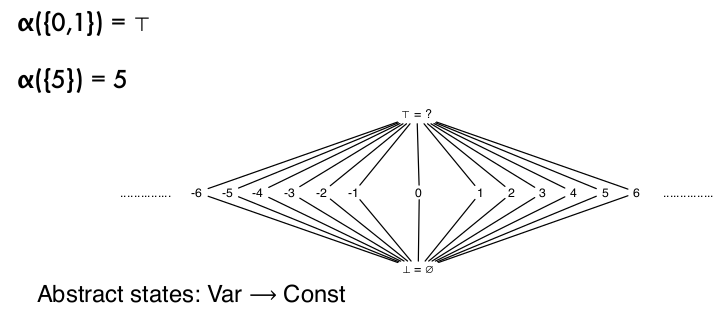
\includegraphics[scale=0.32]{Const}
\end{figure}

Dominio concreto: $\mathbb{V}\rightarrow \mathbb{Z}$

Dominio astratto: $\mathbb{V}\rightarrow \mathcal{P}(\mathbb{Z})$
\newline

\noindent
\underline{\textit{Semantica astratta delle espressioni:}}
\begin{align*}
op &= operatore\\
a ~op~ b &=
\begin{cases}
a ~op~ b &\text{ se a e b sono costanti}\\
\top &\text{ se $a=\top$ $\lor~$ $b=\top$}
\end{cases}\\
\llbracket c \rrbracket^\sharp D &= c\\
\llbracket op~e \rrbracket^\sharp D &= op^\sharp\llbracket e\rrbracket^\sharp D\\
\llbracket e_1~op~e_2 \rrbracket^\sharp D &= \llbracket e_1\rrbracket^\sharp D ~op^\sharp~\llbracket e_2\rrbracket^\sharp D\\
\llbracket x\rrbracket^\sharp D &= D(x)
\end{align*}

\underline{\textit{Semantica astratta dei comandi:}}

$D =$ memoria
\begin{align*}
\llbracket ; \rrbracket^\sharp D &= D\\
\llbracket NonZero(e) \rrbracket^\sharp D &=
\begin{cases}
\bot &\text{ se } \llbracket e\rrbracket^\sharp D = 0 \\
D &\text{ se } \llbracket e\rrbracket^\sharp D \neq 0
\end{cases}\\
\llbracket Zero(e) \rrbracket^\sharp D &=
\begin{cases}
D &\text{ se } 0\subseteq \llbracket e\rrbracket^\sharp D \\
\bot &\text{ se } 0\nsubseteq \llbracket e\rrbracket^\sharp D
\end{cases}\\
\llbracket x\leftarrow e \rrbracket^\sharp D &= D[x\mapsto \llbracket e\rrbracket^\sharp D]\\
\llbracket x\leftarrow M[e] \rrbracket^\sharp D &= D[x\mapsto \top] \text{\hspace{0.5cm} non so cos'è M[e] perché lo valuterò dopo}\\
\llbracket M[e_1]\leftarrow e_2 \rrbracket^\sharp D &= D
\end{align*}

\subsubsection*{Segni}
\addcontentsline{toc}{subsubsection}{Segni}
Dominio rappresentato da un semipiano (un insieme di punti), quindi non va subito a $\top$.

\newpage
\subsubsection*{Intervalli}
\addcontentsline{toc}{subsubsection}{Intervalli}
Il dominio degli Intervalli non è \textit{ACC}, dunque non garantisce la terminazione: per questo viene introdotto il \textit{widening}.

\begin{center}
$[a, b]$ dove $a\leq x\leq b$ (convessi)

$\mathbb{I} = \{[l, u] ~|~ l\in \mathbb{Z}\cup \{-\infty\}, u\in\mathbb{Z}\cup \{+\infty\}, ~l\leq u\}$
\end{center}

\noindent
\textit{\underline{Operazioni astratte}}:
\begin{itemize}
	\item $[l_1, u_1] +^\sharp [l_2, u_2] = [l_1 + l_2, u_1 + U_2]$
	\item $-^\sharp[l, u] = [-u, -l]$
	\item $[l_1, u_1] *^\sharp [l_2, u_2] = [a, b]$ dove:
	\begin{itemize}
		\item $a=min(l_1*l_2, l_1*u_2, l_2*u_1, l_2*u_2)$
		\item $b=max(l_1*l_2, l_1*u_2, l_2*u_1, l_2*u_2)$
	\end{itemize}
	\item $[l_1, u_1] =^\sharp [l_2, u_2] =
	\begin{cases}
	[1, 1] &\text{ se } l_1=l_2=u_1=u_2 (costanti) \\
	[0, 0] &\text{ se } u_1 < l_2 \lor ~u_2 < l_1\\
	[0, 1] &\text{ altrimenti (intervalli uguali che approssimano valori diversi) }
	\end{cases}$
	\item $[l_1, u_1] <^\sharp [l_2, u_2] =
	\begin{cases}
	[1, 1] &\text{ se } u_1<l_2 \\
	[0, 0] &\text{ se } u_2 \leq l_1 \\
	[0, 1] &\text{ altrimenti }
	\end{cases}$
\end{itemize}

\underline{\textit{Semantica astratta:}}

$D : \mathbb{V} \rightarrow \mathbb{I}$
\begin{align*}
\llbracket ; \rrbracket^\sharp D &= D\\
\llbracket NonZero(e) \rrbracket^\sharp D &=
\begin{cases}
\bot &\text{ se } [0, 0] = \llbracket e \rrbracket^\sharp D \\
D &\text{ se } [0, 0] \neq \llbracket e \rrbracket^\sharp D~ \text{ (contiene anche altri valori)}
\end{cases}\\
\llbracket Zero(e) \rrbracket^\sharp D &=
\begin{cases}
D &\text{ se } [0, 0] \subseteq \llbracket e \rrbracket^\sharp D~ \text{ (lo $0$ è uno dei possibili valori)} \\
\bot &\text{ se } [0, 0] \nsubseteq \llbracket e \rrbracket^\sharp D~ \text{ (l'intervallo $e$ non contiene $0$)}
\end{cases}\\
\llbracket x\leftarrow e \rrbracket^\sharp D &= D[x\mapsto \llbracket e\rrbracket^\sharp D]\\
\llbracket x\leftarrow M[e] \rrbracket^\sharp D &= D[x\mapsto [-\infty, +\infty]~~ \text{ (elemento $\top$ degli intervalli)}\\
\llbracket M[e_1]\leftarrow e_2 \rrbracket^\sharp D &= D
\end{align*}




	\chapter*{Analisi Dinamica}
	\addcontentsline{toc}{chapter}{Analisi Dinamica}
	L'analisi dinamica di un programma si basa sulla sua esecuzione e viene utilizzati in vari ambiti: \textit{testing}, \textit{debugging}, \textit{emulation/virtualization}, \textit{profiling/tracing}, \textit{monitoring}, \textit{dynamic slicing}.
	
	Nelle sezioni seguenti ne analizziamo alcuni nel dettaglio.
	
	\section*{Testing}
	\addcontentsline{toc}{section}{Testing}
	Si tratta principalmente dell'esecuzione di un programma basata su un campione di dati (molto piccolo) passato come input.
	
	L'\textbf{obiettivo} è la ricerca di bug/errori/difetti del software, senza correggerli. Questa operazione viene svolta nella fase di testing da professionisti con un'esperienza nella ricerca e identificazione dei bug.
	\newline
	\newline
	\noindent
	Durante la fase di testing si devono ricercare:
	\begin{itemize}
		\item \textbf{mistake}: un'azione umana che ha prodotto un risultato scorretto;
		\item \textbf{fault}: un passaggio scorretto (una definizione di variabile...) all'interno del programma;
		\item \textbf{failure}: la mancata abilità da parte del sistema di svolgere le funzioni richieste;
		\item \textbf{errori}: la differenza tra il valore atteso e il valore effettivamente calcolato/osservato;
		\item \textbf{specifiche}: un documento che specifica, in modo completo e preciso, le richieste e le caratteristiche del sistema e/o dei componenti e spesso delle procedure per verificare quali delle disposizioni sono state soddisfatte.
	\end{itemize}

	\section*{Debugging}
	\addcontentsline{toc}{section}{Debugging}
	
	L'\textbf{obiettivo} è l'identificazione, l'isolamento e la risoluzione dei problemi/bug. Questa operazione si può svolgere durante la fase di sviluppo del software oppure in una fase apposita in cui vengono sistemati i bug riportati dopo i test.
	
	\section*{Program Slicing}
	\addcontentsline{toc}{section}{Program Slicing}
	Si tratta di una tecnica di decomposizione che trasforma un programma originale, cancellandone alcune istruzioni che non hanno alcun effetto sulle \textit{variabili di interesse} nei \textit{punti di interesse}.
	
	Lo \textit{slice} è il programma trasformato secondo il \textit{criterio di slicing} che descrive i parametri di interesse: \textit{V} (insieme delle variabili di interesse) e \textit{n} (punti di interesse del programma).
	
	Ci sono diversi motivi per i quali effettuare il \textit{program slicing}: \textit{program debugging}, \textit{testing} (lo slicing riduce i costi del \textit{regresssion testing} dopo una trasformazione del codice), \textit{parallelizzazione},	\textit{compresione di una programma} (effettuare lo slicing aiuta a comprendere come viene eseguito un programma e quali variabili verranno modificate nei vari percorsi) e \textit{mantenimento del software} (per modificare il codice senza \textit{side effects} indesiderati in giro per il programma).
	\newline
	\newline
	\noindent
	Esistono \textbf{diversi tipi di program slicing}:
	\begin{itemize}
		\item \textit{\textbf{Static slicing}}: l'equivalenza tra programma originale e slice deve, implicitamente, essere valida per ogni possibile input;
		\item \textit{\textbf{Conditioned slicing}}: preserva il significato del programma originale per un insieme di input che soddisfa una particolare condizione $\phi$;
		\item \textit{\textbf{Dynamic slicing}}: considera una particolare computazione, e dunque un particolare input, in modo da preservare il significato del programma unicamente per quell'input.
	\end{itemize}
	
	\noindent
	Esistono, inoltre, \textbf{diverse forme di program slicing}:
	\begin{itemize}
		\item \textit{\textbf{Korel \& Laski} (KL)}: è una forma di slicing molto forte in cui il programma e lo slice devono seguire \textit{paths} identici. Il programma e lo slice hanno la stessa semantica operazionale. Il \textit{path} seguito dallo slice deve essere un \textit{subpath} dell'esecuzione originale.
		\item \textit{\textbf{Iteration Count} (IC)}: richiede che lo slice e il programma si pareggino solo ad una certa iterazione $k$ di un program point $n$ (cioè quando lo statement al program point $n$ viene eseguito per la $k$-esima volta), e non per tutte le iterazioni dello stesso program point.
		\item \textit{\textbf{KL-IC}}(combinazione dei precedenti): richiede che il programma e lo slice seguano \textit{paths} identici e siano uguali solamente ad una particolare iterazione di un certo program point.
	\end{itemize}


	
\end{document}